%============================================================================
% tento soubor pouzijte jako zaklad
% (c) 2008 Michal Bidlo
% E-mail: bidlom AT fit vutbr cz
%============================================================================
% kodovaní: utf-8
%----------------------------------------------------------------------------
% zpracování: make, make pdf, make desky, make clean
% připomínky posílejte na e-mail: bidlom AT fit.vutbr.cz
% vim: set syntax=tex encoding=latin2:
%============================================================================
\documentclass[cover,zadani,print]{fitthesis} % odevzdani do wisu - odkazy, na ktere se da klikat
%\documentclass[cover,print]{fitthesis} % pro tisk - na odkazy se neda klikat
%\documentclass[english,print]{fitthesis} % pro tisk - na odkazy se neda klikat
%      \documentclass[english]{fitthesis}
% * Je-li prace psana v anglickem jazyce, je zapotrebi u tridy pouzit
%   parametr english nasledovne:
%      \documentclass[english]{fitthesis}
% * Neprejete-li si vysazet na prvni strane dokumentu desky, zruste
%   parametr cover

% zde zvolime kodovani, ve kterem je napsan text prace
% "latin2" pro iso8859-2 nebo "cp1250" pro windows-1250, "utf8" pro "utf-8"
%\usepackage{ucs}
\usepackage[czech]{babel}
\usepackage[utf8]{inputenc}
\usepackage[T1]{fontenc}
%\usepackage{fouriernc}
\usepackage{lmodern}
%\usepackage{garamondx}
%\usepackage[garamondx,cmbraces]{newtxmath}
\usepackage{url}
\DeclareUrlCommand\url{\def\UrlLeft{<}\def\UrlRight{>} \urlstyle{tt}}

%zde muzeme vlozit vlastni balicky

\usepackage{graphicx}
\usepackage{epstopdf}
\usepackage{amssymb}
\usepackage{amsmath}
\usepackage{multirow}
\usepackage{array}
\usepackage{enumerate}
\usepackage{enumitem}
\usepackage[normal]{subfigure}
\usepackage{blindtext}
\usepackage[usenames,dvipsnames,svgnames,table]{xcolor}
\usepackage{xfrac}
\usepackage{diagbox}
\usepackage[Algoritmus]{algorithm}
\usepackage{algpseudocode}
\usepackage{multicol}
\usepackage{pdfpages}
\usepackage{pdfsync}

\usepackage[
    backend=biber,      % if we want unicode
    style=iso-numeric, % or iso-numeric for numeric citation method
    babel=other,        % to support multiple languages in bibliography
    sortlocale=cs_CZ,   % locale of main language, it is for sorting
    bibencoding=UTF8,   % this is necessary only if bibliography file is in different encoding than main document
    sorting=nty,
    maxnames=3
]{biblatex}
\bibliography{literatura}

\definecolor{blind}{gray}{0.7}
\newcommand{\blind}[1][\value{blindtext}]{{\color{blind}\blindtext[#1]}}
\newcommand{\Blind}[1][\value{Blindtext}]{{\color{blind}\Blindtext[#1]}}

\definecolor{darkred}{RGB}{127,0,0}
\definecolor{darkgreen}{RGB}{0,127,0}
\definecolor{green}{RGB}{0,220,0}

\colorlet{todo}{red}
\newcommand{\todo}[1]{{\color{todo} {[[#1]]} }}
\newcommand\crule[3][black]{\textcolor{#1}{\rule{#2}{#3}}}
\newcommand\placeholder[1]{{\crule[blind]{\textwidth}{#1}}}

\usepackage[font=small,labelsep=period]{caption}
\setlength{\captionmargin}{20pt}

%\mathchardef\mhyphen="2D


% =======================================================================
% balíček "hyperref" vytváří klikací odkazy v pdf, pokud tedy použijeme pdflatex
% problém je, že balíček hyperref musí být uveden jako poslední, takže nemůže
% být v šabloně
\ifWis
\ifx\pdfoutput\undefined % nejedeme pod pdflatexem
\else
  \usepackage{color}
  \usepackage[unicode,colorlinks,hyperindex,plainpages=false,pdftex]{hyperref}
  \definecolor{links}{rgb}{0.4,0.5,0}
  \definecolor{anchors}{rgb}{1,0,0}
  \def\AnchorColor{anchors}
  \def\LinkColor{links}
  \def\pdfBorderAttrs{/Border [0 0 0] }  % bez okrajů kolem odkazů
  \pdfcompresslevel=9
\fi
\fi

%Informace o praci/projektu
%---------------------------------------------------------------------------
\projectinfo{
  %Prace
  project=SP,            %typ prace BP/SP/DP/DR
  year=2015,             %rok
  date=\today,           %datum odevzdani
  %Nazev prace
  title.cs={Souběžné učení v koevolučních algoritmech},  %nazev prace v cestine
  title.en={Colearning in Coevolutionary Algorithms}, %nazev prace v anglictine
  %Autor
  author={Michal Wiglasz},   %jmeno prijmeni autora
  author.title.p=Bc., %titul pred jmenem (nepovinne)
  %author.title.a=PhD, %titul za jmenem (nepovinne)
  %Ustav
  department=UPSY, % doplnte prislusnou zkratku: UPSY/UIFS/UITS/UPGM
  %Skolitel
  supervisor={Michaela Šikulová}, %jmeno prijmeni skolitele
  supervisor.title.p=Ing.,   %titul pred jmenem (nepovinne)
  %supervisor.title.a={Ph.D.},    %titul za jmenem (nepovinne)
  zadaniPdf={../zadani-bw.pdf}
}

%Abstrakt (cesky, anglicky)
\abstract[cs]{Kartézské genetické programování je druh genetického programování, ve kterém jsou kandidátní programy reprezentovány jako orientované acyklické grafy. Bylo ukázáno, že je možné evoluci urychlit použitím koevoluce, kde se ve druhé populaci vyvíjí prediktory fitness. Prediktory fitness slouží k přibližnému určení kvality kandidátních řešení. Nevýhodou koevolučního přístupu je nutnost provést mnoho časově náročných experimentů pro určení nejvýhodnější velikosti prediktoru pro daný problém. V této práci je představena nová reprezentace prediktorů fitness s plastickým fenotypem, založená na principech souběžného učení v evolučních algoritmech. Plasticita fenotypu umožňuje odvodit různé fenotypy ze stejného genotypu. Díky tomu je možné adaptovat velikost prediktoru na současný průběh evoluce a obtížnost řešeného problému. Navržený algoritmus bude implementován v navazující diplomové práci a vyhodnocen na úloze návrhu obrazových filtrů.}

\abstract[en]{Cartesian genetic programming (CGP) is a form of genetic programming where candidate programs are represented in the form of directed acyclic graphs. It was shown that CGP can be accelerated using coevolution with a population of fitness predictors which are used to estimate the quality of candidate solutions. The major disadvantage of the coevolutionary approach is the necessity of performing many time-consuming experiments to determine the best size of the fitness predictor for the particular task. This project introduces a new fitness predictor representation with phenotype plasticity, based on the principles of colearning in evolutionary algorithms. Phenotype plasticity allows to derive various phenotypes from the same genotype. This allows to adapt the size of the predictors to the current state of the evolution and difficulty of the solved problem. The proposed algorithm will be implemented as a part of the master's thesis and it will be evaluated in the task of evolutionary image filter design.}

%Klicova slova (cesky, anglicky)
\keywords[cs]{Koevoluční algoritmus, kartézské genetické programování, evoluční algoritmus, Baldwinův efekt, plasticita fitness, predikce fitness, zpracování obrazu.}
\keywords[en]{Coevolutionary alghorithm, cartesian genetic programming, evolutionary algorithm, Baldwin effect, fitness plasticity, fitness predictor, image processing.}

%Prohlaseni
\declaration{Prohlašuji, že jsem tento semestrální projekt vypracoval samostatně pod vedením Ing. Michaely Šikulové. Uvedl jsem všechny literární prameny a publikace, ze kterých jsem čerpal.}

%Podekovani (nepovinne)
\acknowledgment{Rád bych poděkoval Ing. Michaele Šikulové za cenné rady, podnětné konzultace a odbornou pomoc při řešení této práce.}

\begin{document}
  % Vysazeni titulnich stran
  % ----------------------------------------------
  \maketitle
  % Obsah
  % ----------------------------------------------
  \setcounter{secnumdepth}{2}
  %\setcounter{tocdepth}{1}
  \tableofcontents

  % Seznam obrazku a tabulek (pokud prace obsahuje velke mnozstvi obrazku, tak se to hodi)
  % \listoffigures
  % \listoftables

  % Text prace
  % ----------------------------------------------
  % -*- root: projekt.tex -*-
%=========================================================================
% (c) Michal Bidlo, Bohuslav Křena, 2008

\chapter{Úvod}

\blind

%% \section{Obrazové filtry}

Tato zpráva je strukturována následovně: Kapitola 2 se zabývá evolučními algoritmy, zejména kartézským genetickým programováním, použitím koevoluce za účelem snížení výpočetní náročnosti a souběžným učením. Kapitola 3 se zabývá návrhem programu pro tvorbu obrazových filtrů použitím koevolučního algoritmu se souběžným učením, který bude implementován v~diplomové práci.

\chapter{Evoluční algoritmy}

První evoluční algoritmy se v~literatuře objevují od 50. let 20. století. Postupně a nezávisle na sobě vzniklo několik podobných evolučních metod (například evoluční strategie, evoluční programování nebo genetické algoritmy), které se v~různých obměnách používají i dnes. Až s~rozšířením spolupráce mezi těmito nezávislými výzkumnými týmy v~90. letech vznikl pojem \uv{evoluční algoritmus}.

Evoluční algoritmy jsou stoachastické optimalizační metody inspirované přírodou, konkrétně Darwinovou teorií evoluce. Ačkoliv pojmy používané v~evolučních algoritmech vycházejí z~biologie, jejich význam není vždy přesně stejný. Mezi základní pojmy patří:

\begin{itemize}
    \item\emph{Gen} je základním stavebním blokem kandidátního řešení, je omezen předem danou abecedou (binární čísla, písmena\ldots),
    \item\emph{Alela} je konkrétní hodnota genu,
    \item\emph{Chromozom}, \emph{jedinec} nebo \emph{genotyp} je posloupnost genů kódující kandidátní řešení,
    \item\emph{Fenotyp} je dekódovaný genotyp,
    \item\emph{Populace} je konečná množina chromozomů,
    \item\emph{Fitness} udává \uv{kvalitu} jedince s~ohledem na řešený problém,
    \item\emph{Fitness funkce} přiřazuje každému jedinci hodnotu fitness,
    \item\emph{Diverzita} udává rozmanitost populace, tj. nakolik se od sebe chromozomy v~populaci navzájem liší,
    \item\emph{Rodiče} jsou podmnožina populace, ze které budou vytvořeni \emph{potomci}.
\end{itemize}

Typickým rysem evolučních algoritmů je to, že pracují s~populací několika kandidátních řešení, od kterých odvozují nová řešení pomocí speciálních biologií inspirovaných operátorů. Jednoduchý evoluční algoritmus lze zapsat takto:

\begin{enumerate}
    \item Náhodně vygeneruj populaci o~dané velikosti.
    \item Opakuj dokud není splněna ukončovací podmínka:
    \begin{enumerate}
        \item z~populace vyber rodiče a vytvoř potomky,
        \item některé jedince v~populaci nahraď potomky.
    \end{enumerate}
    \item Výsledkem je jedinec s~nejvyšší fitness (nejlepší nalezené řešení problému).
\end{enumerate}

Nevýhodou evolučních algoritmů je velké množství parametrů a podproblémů. Před samotným výpočtem pomocí evolučního algoritmu je třeba si položit například tyto otázky:

\begin{itemize}
    \item Jak se budou kódovat kandidátní řešení do genotypu?
    \item Kolik jedinců má být v~populaci?
    \item Jak se budou vybírat rodiče nové populace?
    \item Jak se budou tvořit potomci?
    \item Kolik jedinců v~populaci má být nahrazeno potomky?
\end{itemize}

Je třeba brát v~potaz i jejich stochastickou povahu, z~čehož plyne, že pro porovnání různých algoritmů (nebo různých hodnot parametrů) je potřeba statisticky vyhodnotit větší množství běhů \cite{HandbookEA, Modra}.

\section{Genetický algoritmus}
\label{secGA}

Genetický algoritmus byl vytvořen Johnem Hollandem v~sedmdesátých letech. Samotný termín \uv{genetický algoritmus} se začal běžně používat až po publikaci dizertační práce Kena De Jonga v~roce 1975. Do širšího povědomí se dostává v~půlce osmdesátých let, kdy se ukázalo, že jej lze použít k~řešení řadě obtížných úloh.

%Existují i hybridní genetické algoritmy, ve kterých se uplatňuje lokální prohledávání.

Schéma genetického algoritmu odpovídá obecnému evolučnímu algoritmu. Počáteční populace je vytvořena náhodně. V~každé iteraci se populace ohodnotí (určí se fitness jedinců) a podle zvoleného selekčního algoritmu se vyberou rodiče, ze kterých jsou pomocí operátorů křížení a mutace vytvořeni potomci. Kromě potomků je možné v~nové populaci zachovat i několik jedinců z~původní populace (s~případnou mutací). Pokud se používá \emph{elitismus}, je nejlepší jedinec vždy součástí nové populace \cite{HandbookEA, Modra}.


\subsection{Reprezentace řešení}

Genotyp v~genetickém algoritmu je často jednoduchá datová struktura, jako je pole bitů nebo čísel konstantní délky. V~případně binárního chromozomu může být vhodné použít Grayovo kódování, ve kterém se dvě po sobě jdoucí hodnoty liší vždy pouze jedním bitem. To pomáhá překonat tzv. Hammingovu bariéru, kdy malá změna v~genotypu způsobí velkou změnu ve fenotypu a naopak.


\subsection{Selekce rodičů}

Volbu $K$ rodičů z~populace lze provést několika způsoby. Nejjednodušší je prosté seřazení jedinců podle jejich fitness, rodiči se pak stává $K$ jedinců s~nejvyšší fitness.

U~\emph{proporciální selekce} je pravděpodobnost, že se konkrétní jedinec stane rodičem, přímo úměrná jeho fitness:

\begin{equation*}
p_i = \frac{f_i}{\sum_{j=1}^N{f_j}}
\end{equation*}

\noindent{}Lze si to představit jako ruletu, kde každá výseč odpovídá jednomu jedinci a čím vyšší má tento jedinec fitness, tím je výseč větší. Pokud má ale jeden nebo více jedinců výrazně vyšší fitness než zbytek, zmenšuje se diverzita populace -- rodiči se téměř vždy stávají titíž jedinci. Jedním ze způsobů, jak se tento problém řeší je, že se jedinci seřadí podle velikosti fitness a pravděpodobnost výběru je úměrná pořadí jedince a ne přímo jeho fitness.

Jiným přístupem k~výběru rodičů je \emph{turnajová selekce}. Do turnajového kola je náhodně zvoleno dva nebo více jedinců. Vítězem kola se stává jedinec s~nejvyšší fitness a ten se stává rodičem. Turnaj se opakuje tolikrát, kolik rodičů je potřeba zvolit \cite{Modra}.


\subsection{Křížení}

Křížení je stěžejním bodem genetického algoritmu. Během něj jsou kombinovány geny ze dvou nebo více chromozomů, čímž vznikne nový jedinec. Obrázek \ref{obrKrizeni} znázorňuje tři základní mechanismy: jednobodové, vícebodové a uniformní křížení. U~jednobodového křížení je náhodně zvolen bod, ve kterém se chromozomy rozdělí a geny za tímto bodem si mezi sebou vymění. U~vícebodového křížení je těchto bodů několik a je možné geny promíchat důkladněji. V~případě uniformního křížení se rozhoduje, zda dojde k~prohození nebo ne, u~každého genu zvlášť \cite{Modra}.

\begin{figure}[htb]
    \centering
    \subfigure[Jednobodové]{
        \centering
            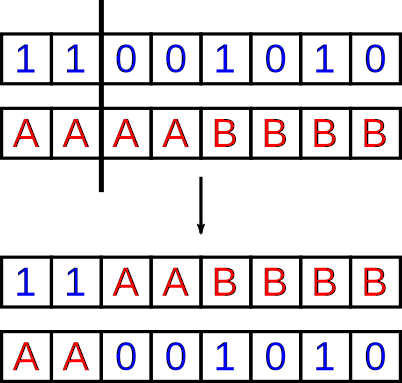
\includegraphics[width=0.27\textwidth]{fig/crossover1.pdf}
    }
    \subfigure[Vícebodové]{
        \centering
            \includegraphics[width=0.27\textwidth]{fig/crossover2.pdf}
        }
    \subfigure[Uniformní]{
        \centering
            \includegraphics[width=0.27\textwidth]{fig/crossoverU.pdf}
        }
    \caption{Tři základní mechanismy křížení v~genetickém algoritmu.}
    \label{obrKrizeni}
\end{figure}


\subsection{Mutace}

Mutace je malá změna genotypu, která se s~malou pravděpodobností provádí u~potomků vzniklých křížením. V~případě binárně kódovaného chromozomu mutace spočívá v~překlopení několika náhodně zvolených bitů. U~celočíselného kódování je hodnota genu nahrazena náhodným číslem. Pokud je z~povahy problému hodnota genu omezená výčtem nebo intervalem, je vhodné, aby výsledkem mutace nebyla nepřípustná hodnota. \cite{Modra}.

\section{Kartézské genetické programování}
\label{secCGP}

Další variantu evolučního algoritmu, genetické programování, představil koncem 80. let 20. století John Koza. Zabývá automatizovanou tvorbou celých programů, kdy neřeší jak má program pracovat, pouze co má být jeho výstupem. John Koza pracoval s~jazykem LISP, pro který je vhodná reprezentace programu pomocí stromů, existují ale i jiné způsoby kódování programů do chromozomu, například kartézské genetické programování (CGP), které vytvořil Julian Miller koncem devadesátých let.

V~kartézském genetickém programování se programy kódují jako orientované acyklické grafy, reprezentované dvourozměrnou kartézskou mřížkou výpočetních uzlů (funkčních bloků) o~předem daných rozměrech $n_c \times n_r$ (viz obrázek \ref{obrCGP}). Počet primárních vstupů $n_i$ a výstupů $n_o$ je fixní. Každý výpočetní uzel vykonává nějakou funkci z~předem daného seznamu. Pro různé problémy je vhodné používat odpovídající funkce, například pro tvorbu logických obvodů to jsou dostupná logická hradla, pro symbolickou regresi to mohou být aritmetické operace apod. Vstupy funkčních bloků jsou napojeny buď na některý z~primárních vstupů, nebo na výstup uzlu umístěného v~některém sloupci nalevo. O~kolik sloupců doleva je možné uzly propojovat určuje parametr $l$-back. Pokud je roven jedné, je možné propojovat pouze uzly ze sousedních sloupců, pokud je $l$-back roven počtu sloupců $n_c$, lze uzly propojovat libovolně. Zpětné vazby a cykly nejsou v~CGP povoleny.

\begin{figure}[htb]
    \centering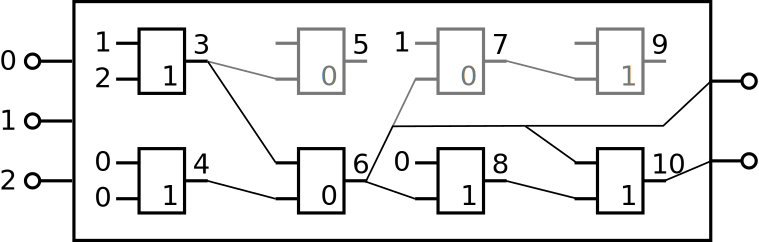
\includegraphics[width=0.8\textwidth]{fig/cgp.pdf}
    \caption{Program v~kartézském genetickém programování. Uzly 5, 7 a 9 jsou neaktivní.}
    \label{obrCGP}
\end{figure}

Chromozom je pak posloupnost celých čísel konstantní délky, jednotlivé geny určují propojení a funkci výpočetních uzlů. Na konci chromozomu je pro každý primární výstup jeden gen obsahující číslo uzlu, jehož výstup má být použit. Oproti genotypu je velikost fenotypu variabilní, protože některé výpočetní uzly mohou zůstat nepoužité, pokud nejsou propojeny přímo či nepřímo na primární výstupy programu. Takovým uzlům se říká \emph{neaktivní bloky}. Nikdy ale nepřesáhne velikost genotypu. Výhodou je omezený prohledávací prostor, nehrozí tak jako u~stromové reprezentace, že by délka programu během evoluce rostla nad únosnou mez. Ten lze dále omezovat parametrem $l$-back a omezením množiny dostupných funkcí \cite{ZelenaCGP, Modra}.


\subsection{Průběh evoluce}
\label{secCGPEvo}

Schéma evoluce opět odpovídá obecnému evolučnímu algoritmu. Počáteční populace je opět vygenerována náhodně. Oproti genetickému algoritmu kartézské genetické programování nepoužívá křížení. Po ohodnocení všech jedinců je nejlepší z~nich určen rodičem. Ostatní jedinci jsou nahrazeni náhodnými mutacemi rodiče.

Mutace mění náhodně hodnotu některých genů jedince. Jejich počet se běžně volí jako procento z~celkového počtu genů, označované jako \emph{míra mutace} $\mu_r$. Geny nelze nahrazovat libovolnými hodnotami, je třeba brát ohled na parametr $l$-back, počet primárních vstupů a počet dostupných funkcí pro výpočetní uzly:

\begin{itemize}
    \item U~genu kódující funkci, je náhodně vygenerován index funkce ze seznamu dostupných funkcí.
    \item U~genu kódující vstup funkčního bloku jsou povolenými hodnotami:
        \begin{itemize}
            \item číslo primárního vstupu programu (0 až $n_i$),
            \item číslo některého uzlu ze sloupců nalevo -- s~ohledem na parametr $l$-back.
        \end{itemize}
    \item U~genu kódující primární výstup je náhodně vybráno číslo některého výpočetního uzlu nebo primárního vstupu.
\end{itemize}

Ne každá mutace vede na změnu fenotypu -- může dojít například ke změně funkce funkčního bloku nepřipojeného na výstup nebo propojení mezi neaktivními bloky, popř. může dojít ke změně v~aktivní části programu, která ale nemá vliv na jeho funkci. Ukazuje se ale, že i tyto \emph{neutrální mutace} jsou prospěšné pro funkci algoritmu. Proto pokud je v~populaci několik nejlepších jedinců se stejnou hodnotou fitness, je vhodné vybírat jako rodiče toho, který nebyl rodičem v~předchozí generaci, tj. chromozom, který byl odvozen z~předchozího rodiče neutrální mutací. V~opačném případě, kdy se jako rodič použije pouze za jedinec s~vyšší hodnotou fitness, evoluce nachází méně kvalitní programy \cite{ZelenaCGP, Modra}.


\subsection{Výpočet fitness}

K~vyhodnocení fitness jedince je třeba projít všechny prvky testovací množiny. Každý z~nich se skládá ze dvou částí -- vstupních hodnot, které se přiloží na primární vstupy kartézského programu, a očekávané výstupní hodnoty. Protože výpočet fitness je časově nejnáročnější částí evoluce, je vhodné mít množinu trénovacích dat co nejmenší. Samotný výpočet lze provádět \uv{zleva doprava}, kdy jsou postupně vypočítávány výstupy všech funkčních bloků, bez ohledu na to, zda jsou použity ve fenotypu nebo ne. Druhou možností, kdy se pracuje pouze s~aktivními bloky, je postupovat rekurzivním sestupem od výstupů programu ke vstupům. Nevýhodou je, že některé uzly se mohou vyhodnotit vícekrát. Nabízí se oba přístupy zkombinovat, kdy se směrem od výstupů nejprve určí, které bloky jsou aktivní, a poté se směrem od vstupů programu vypočítají výstupy těchto bloků a tím i výstupy celého programu.

\section{Návrh obrazových filtrů evolučními algoritmy}
\label{secIF}

Jedním z~problémů, který lze řešit pomocí evolučních algoritmů je návrh obrazových filtrů, které se používají jako jeden z~prvních kroků u~zpracování obrazových dat. Čím lépe filtr dokáže obnovit poškozené části obrazu, tím lepší výsledky lze získat v~dalších krocích algoritmu, jako je například segmentace nebo klasifikace.

Většina hardwarových i softwarových implementací obrazových filtrů pracuje s~lokálním okolím pixelů, nejčastěji jde o~9-okolí nebo 25-okolí. Novou hodnotu pixelu určuje funkce, na jejímž vstupu jsou hodnoty všech pixelů ve zvoleném okolí. Tato funkce se postupně aplikuje na celý obrázek. Tento princip znázorňuje obrázek \ref{obrIFokoli}.

\begin{figure}[htb]
    \centering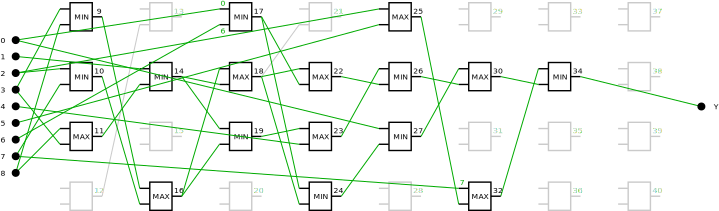
\includegraphics[width=0.85\textwidth]{fig/filter.pdf}
    \caption{Princip filtrace obrazu.}
    \label{obrIFokoli}
\end{figure}

Existují různé typy šumů, pro které jsou vhodné různé typy obrazových filtrů. Poměrně častý je impulzní šum, který vzniká kvůli nefunkčním pixelům v~kameře, chybným paměťovým buňkám nebo chybám při přenosu dat. Poškozené body mají buď náhodnou hodnotu (výstřelový šum) nebo mají vždy minimální nebo maximální možnou hodnotu (šum typu sůl a pepř). Pro výstřelový šum je vhodný mediánový filtr, u~kterého je opravená hodnota pixelu určena jako medián jeho okolí, jeho nevýhodou je ztráta detailů nedostatečná kvalita výstupu při intenzivnějším šumu-

Evoluční algoritmy lze při návrhu obrazových filtrů použít různými způsoby. Jednou možností je vzít již existující obrazový filtr, u~nějž se pomocí genetického algoritmu optimalizuje nastavení jeho parametrů tak, aby se dosáhlo co nejlepších výsledků v~zamýšleném prostředí. Evoluční algoritmy lze použít také přímo pro návrh nových obrazových filtrů. Zvláště výhodné je to u~nelineárních filtrů, pro jejichž analýzu a návrh schází vhodný matematický aparát a jejich tvorba je tak obtížnější než v~případě lineárních filtrů.

Jako vhodné pro tuto úlohu se ukazuje kartézské genetické programování \cite{ZelenaIF}. Na vstup kartézského programu je přivedeno zvolené okolí pixelu, výstupem je vyfiltrovaný pixel. Jako fitness funkce se nejčastěji používá špičková hodnota poměru signál/šum v~decibelech (Peak Signal to Noise Ratio, PSNR) nebo v~hardware snáze implementovatelná střední odchylka pixelů (Mean Difference Per Pixel, MDPP). Tyto funkce jsou definovány jako:

\begin{equation}
    \label{eqPSNR}
    \mathit{PSNR} = 10 \log_{10} \frac{255^2}{\frac{1}{MN} \sum\limits_{i,j} \left( v\left( i, j \right) - w\left( i, j \right)  \right)^2 }
\end{equation}

\begin{equation}
    \label{eqMDPP}
    \mathit{MDPP} = \frac{1}{MN} \sum\limits_i^M \sum\limits_j^N \left| v\left( i, j \right) - w\left( i, j \right) \right|
\end{equation}

\noindent{}kde $M$ a $N$ označují rozměry obrázku, $v$ vyfiltrovaný a $w$ původní obrázek.

Pro výpočet fitness kandidátního filtru musíme zpracovat celý obrázek, kdy každý pixel můžeme považovat za jeden případ fitness. Protože i pro poměrně malé obrázky jich je několik tisíc, je výpočet fitness časově velmi náročný.

\section{Koevoluce v~kartézském genetickém programování}

Jedním ze způsobů, jak řešit problém velkého množství případů fitness je použití koevolučního algoritmu. Oproti dosud zmíněným evolučním algoritmům zde existuje několik různých populací, které na sebe navzájem působí a ovlivňují svůj vývoj. Fitness jedince nezávisí pouze na jeho genetických předpokladech, ale určuje se podle toho, jak \uv{dobrý} je při interakci s~jedinci z~jiných populací.

Populace mohou být stejného druhu, které jsou navzájem oddělené bariérou a vyvíjejí se nezávisle na sobě až na občasné interakce, kdy někteří jedinci migrují mezi podpopulacemi, například pokud některá z~nich uvízne v~lokálním extrému. V~některých případech je vhodné mít několik populací různého druhu. Některé složitější problémy lze dekomponovat na několik jednodušších, které mohou být reprezentovány různými chromozomy. Jedinci spolu spolupracují na řešení úlohy a jejich kvalita závisí na kvalitě ostatních jedinců. V~tomto případě mluvíme o~\emph{kooperativní koevoluci}.

Další variantou je \emph{soutěživá koevoluce}, pro tzv. úlohy založené na testu. Populace mezi sebou interagují prostřednictvím fitness funkce, jejíž výstupy pro jednu populaci jsou ovlivněny jedinci z~druhé populace; typicky jsou jedinci jedné populace ohodnocování pomocí nejlepšího nebo několika nejlepších jedinců z~druhé populace. Pro tyto účely bývá součástí algoritmu jeden nebo více \emph{archivů}, do kterých jsou umisťování nejlepší nalezení jedinci.

Z~implementačního hlediska je možné vyhradit pro každou z~populací samostatné vlákno nebo proces, které mezi sebou komunikují zasíláním zpráv nebo přes sdílenou paměť. Není to ale nutné, koevoluci lze modelovat také tak, že v~každé iteraci algoritmu proběhne několik generací v~první populaci, poté několik generací ve druhé populaci.

Použitím koevoluce lze řešit zmíněný problém velkého množství případů fitness v~úloze návrhu obrazových filtrů vytvořením druhé populace, která vybírá vhodnou podmnožinu pixelů, která slouží k~výpočetu fitness kandidátních filtrů.


\subsection{Koevoluční řešení symbolické regrese}

Koevoluční výpočet za účelem snížení výpočetní náročnosti byl poprvé úspěšně použit na úloze symbolické regrese \cite{SikuEuroGP}. Zde jsou použity dvě populace: populace kartézských programů (kandidátních řešení symbolické regrese) a populace tzv. prediktorů fitness. Prediktory určují podmnožinu trénovacích dat, která má být použita k~ohodnocení kandidátních programů. Kromě těchto populací je součástí řešení archiv sdílený oběma populacemi, který obsahuje několik kartézských programů. Celé schéma populací a interakcí mezi nimi znázorňuje obrázek \ref{obrKoevoluce}.

\begin{figure}[htb]
    \centering\includegraphics[width=\textwidth]{fig/coevolution.pdf}
    \caption{Schéma koevoluce CGP a prediktorů fitness \cite{SikuEuroGP}.}
    \label{obrKoevoluce}
\end{figure}

Evoluce kandidátních programů probíhá pomocí kartézského genetického programování. Ve skutečnosti existují dvě různé fitness funkce: $f_{\mathit{exact}}$, ve které byla použita celá trénovací množina, a $f_{\mathit{predicted}}$, omezená pouze na některé případy fitness. Označíme-li kandidátní program jako $s$, velikost trénovací množiny jako $k$ a délku prediktoru fitness (velikost podmnožiny trénovacích dat) jako $m$, můžeme je zapsat jako:

\begin{equation}
    \label{eqFexact}
    f_{\mathit{exact}} \left( s \right) = \frac{1}{k} \sum\limits_{j=1}^{k} g \left( y \left( j \right) \right)
\end{equation}

\begin{equation}
    \label{eqFpredicted}
    f_{\mathit{predicted}} \left( s \right) = \frac{1}{m} \sum\limits_{j=1}^{m} g \left( y \left( j \right) \right)
\end{equation}

Pokud je během evoluce nalezen jedinec s~lepší predikovanou fitness (vypočtenou funkcí $f_{\mathit{predicted}}$) než nejlepší jedinec v~předchozí generaci, je umístěn do archivu sdíleného s~populací prediktorů. Ten je rozdělen na dvě části -- první z~nich obsahuje nejlepší nalezená řešení, do druhé části jsou pravidelně umisťovány náhodně vygenerované programy, čímž je zajištěna větší diverzita jedinců v~archivu. Každý jedinec umístěný do archivu je ohodnocen pomocí celé trénovací množiny (funkcí $f_{\mathit{exact}}$).

Evoluce prediktorů fitness je řízena genetickým algoritmem. Chromozom má podobu pole ukazatelů do trénovací množiny o~konstantní délce. Potomci jsou tvořeni pomocí jednobodového křížení a mutace, navíc nejhorší jedinec v~populaci je nahrazen náhodně vygenerovaným jedincem. Fitness prediktoru je určena jako střední absolutní odchylka skutečné a predikované fitness všech jedinců v~archivu:

\begin{equation}
    \label{eqFpredictorSR}
    f \left( p \right) = \frac{1}{u} \sum\limits_{i=1}^{u} \left| f_{\mathit{exact}} \left( s \left( i \right) \right) - f_{\mathit{predicted}} \left( s \left( i \right) \right) \right|
\end{equation}



\noindent{}kde $p$ označuje prediktor a $u$ počet jedinců v~archivu. Prediktor s~nejnižší odchylkou je pak použit pro ohodnocování řešení z~populace kartézských programů.

V~článku \cite{SikuEuroGP} byl tento koevoluční algoritmus porovnán s~běžným CGP na pěti různých funkcích, kdy trénovací množina pro každou z~nich obsahovala 200 funkčních bodů. Ukázalo se, že koevolucí lze nalézt přijatelné řešení s~použití mnohem menšího počtu evaluací kandidátních programů než u~standardního CGP. Také se ukázalo, že zatímco standardní CGP nenalezlo přijatelné řešení v~23,6\,\% běhů, koevoluční algoritmus byl úspěšný ve všech případech. Co se výpočetní náročnosti týče, byl koevoluční přístup přibližně dvakrát až pětkrát rychlejší, podle hledané funkce.


\subsection{Koevoluční návrh obrazových filtrů}
\label{secCoevIF}

Podobně jako symbolickou regresi lze pomocí koevoluce akcelerovat i evoluční návrh obrazových filtrů. Opět existují dvě populace, kandidátních filtrů v~CGP a podmnožin případů fitness, také je použit sdílený archiv obrazových filtrů. Jednotlivé položky trénovacích dat jsou složeny z~devítiokolí poškozeného pixelu a hodnoty téhož pixelu v~původním obrázku (což je očekávaný výstup filtru).

V~článku \cite{SikuPPSN} jsou zmíněny dva různé koevoluční přístupy. V~prvním případě šlo o~koevoluci s~prediktory fitness (CFP, coevolution of fitness predictors), podobně jako u~řešení symbolické regrese popsané výše. Fitness filtrů byla určena pomocí funkce MDPP (viz rovnice \ref{eqMDPP}), fitness prediktorů pak jako:

\begin{equation}
    \label{eqFpredictorIF}
    f_{\mathit{CFP}} \left( p \right) = \frac{1}{T} \sum\limits_{i=1}^{T} \left| \mathit{MDPP_{exact}} \left( s \left( i \right) \right) - \mathit{MDPP_{partial}} \left( s \left( i \right) \right) \right|
\end{equation}

\noindent{}kde $T$ označuje počet položek v~archivu filtrů a $\mathit{MDPP_{partial}}$ je střední odchylka podmnožiny pixelů určených prediktorem:

\begin{equation}
    \label{eqMDPPPartial}
    \mathit{MDPP_{partial}} = \frac{1}{K} \sum\limits_l^K \left| v\left( l \right) - w\left( l \right) \right|
\end{equation}

\noindent{}kde $K$ označuje počet případů fitness, $v$ vyfiltrovaný a $w$ původní obrázek. Cílem evoluce prediktorů je minimalizace hodnoty fitness.

Ve druhém případě je použita soutěživá koevoluce (CC, competitive coevolution). Podmnožiny případů fitness zde neslouží jako prediktory fitness, ale jako testy. Na populaci filtrů lze nahlížet jako na \uv{hostitele} a na testy jako na \uv{parazity}. Cílem filtrů je správně vyřešit všechny případy fitness obsažené v~testu, cílem populace testů je najít takové případy fitness, které nalezené filtry nejsou schopny vyřešit správně.
Cílem evoluce testů je tedy nalezení podmnožiny pixelů s~maximalní střední odchylkou, fitness funkci lze odvodit z~rovnice \ref{eqMDPPPartial} následovně:

\begin{equation}
    \label{eqFtestsIF}
    f_{\mathit{CC}} = \frac{1}{T} \sum\limits_{i=1}^{T} \frac{1}{K} \sum\limits_l^K \left| v\left( l \right) - w\left( l \right) \right|
\end{equation}

Podobně jako u~prediktorů je nejlepší nalezený test použit pro ohodnocení populace filtrů. V~obou variantách jsou nejlepší nalezené filtry umisťovány do archivu, který pak slouží k~ohodnocování prediktorů či testů.

V~porovnání se standardním CGP bylo dosaženo přijatelné kvality filtrů při použití podmnožiny případů fitness o~velikosti pouze 15\,\% celkového počtu pixelů v~obrázku. V~tomto případě byl koevoluční výpočet přibližně třikrát rychlejší než standardní CGP. Oba zmíněné koevoluční přístupy (prediktory fitness i soutěživá koevoluce) vykazují podobné výsledky \cite{SikuPPSN}.

\subsection{Akcelerace koevolučního návrhu v~hardware}

Koevoluční CGP bylo také úspěšně implementováno v~hardware na rekonfigurovatelném obvodu (FPGA). Tato implementace byla testována na úloze návrhu obrazových filtrů, kdy byl měřen čas potřebný na dosažení 10~000 generací CGP. Největšího zrychlení bylo dosaženo při použití chromozomů o~délce 25\,\% všech případů fitness, kdy bylo dosaženo 58násobné zrychlení oproti optimalizované\footnote{Pomocí OpenMP a vektorových (SIMD) instrukcí z~instrukční sady SSE 4.1.} softwarové implementaci \cite{Hrbacek}.

\subsection{Návrh obrazových filtrů pomocí kompoziční koevoluce}

Jiným přístupem ke koevolučnímu návrhu je použití kompoziční koevoluce. K~samotnému filtru je možné přidat detektoru šumu, který rozhoduje, zda je právě zpracovávaný pixel poškozený a má být opraven. Cílem je pak nalézt nejlepší kombinaci filtru a detektoru šumu. Experimentálně bylo ověřeno, že koevoluční algoritmus vede na kvalitnější filtry oproti samostatné evoluci filtrů a detektorů šumu bez vzájemné interakce \cite{SikuKomjathy}.

\subsection{Otevřené problémy koevoluce}
\label{secProblems}

Jak bylo ukázáno, použitím koevoluce lze zkrátit dobu potřebnou pro nalezení přijatelného řešení, v~některých případech až pětinásobně, a dokonce koevoluce poměrně spolehlivě nachází řešení v~případech, kdy standardní CGP selhává. Na druhou stranu je zapotřebí poměrně velké množství běhů k~nalezení ideálního nastavení. Kromě velikosti populací, počtu kandidátních řešení v~archivu jde zejména o~délku chromosomu v~populaci podmnožin případů fitness, kdy se pro různé úlohy je vhodné jiné nastavení. Při suboptimální konfiguraci pak nemusí být dosaženo takového urychlení výpočtu, jako by bylo možné, anebo kvalita nalezených řešení nemusí být přijatelná. Například v~případě úlohy symbolické regrese bylo potřeba provést více než sto tisíc nezávislých běhů \cite{SikuEuroGP}, než bylo nalezeno nejvhodnější nastavení.

Pokud jsou v~genetickém algoritmu použity dlouhé chromozomy čítající tisíce genů, vyvstává problém škálovatelnosti. U~evolučních algoritmů se pod tímto problémem rozumí situace, kdy evoluce nenachází přijatelná řešení pro rozsáhlejší úlohy, ačkoliv v~menším měřítku funguje dobře \cite{SikuKomjathy}. Tento problém se výrazně projeví například u~permutačně kódovaného chromozomu, kdy se používají speciální genetické operátory modifikující pouze pořadí jednotlivých genů a ne jejich hodnoty.

\subsection{Nepřímo kódované prediktory fitness}
\label{secIndirectPredictors}

Jedním ze způsobů, jak obejít nutnost najít nejvhodnější délku prediktoru pro konkrétní úlohu, je jejich nepřímé kódování, které evoluci umožní tvořit prediktory různé délky a adaptovat je na konkrétní trénovací data. Prediktory pak nejsou reprezentovány jako obyčejné pole ukazatelů do trénovací množiny, ale jako funkce generující posloupnost ukazatelů, které se mají použít.

Pro hledání vhodné funkce je možné použít kartézské genetické programování. Funkce je reprezentována jako program s~jedním vstupem a dvěma výstupy. Součástí chromozomu je oproti standardnímu CGP ještě hodnota $x_0$ udávající první vstup programu, pomocí kterého je získán první prvek posloupnosti. Jeden z~výstupů slouží jako další prvek posloupnosti (a zároveň jako nový vstup programu), druhý pak udává, zda má být posloupnost ukončena. Fitness generátoru závisí kromě odchylky predikované a skutečné fitness také na délce generované posloupnosti -- delší posloupnost vede na větší výpočetní náročnost.

Během experimentů na úloze symbolické regrese se ukázalo, že počet použitých případů fitness odpovídá počtu zjištěnému experimentálně s~přímo kódovanými prediktory, čili že je možné použít koevoluci s~prediktory fitness na nové úlohy bez pracného hledání optimálního nastavení \cite{Siku2015}.


\section{Souběžné učení v~evolučních algoritmech}

Vztahem mezi učením a evolucí se zabýval už James Mark Baldwin na konci 19. století. Ve svém článku \cite{Baldwin} se zabýval vývojem komplexního instinktivního chování. Tzv. \emph{Baldwinův efekt} popisuje, jakým způsobem lze postupným vývojem po menších krůčcích dosáhnout komplexních instinktů zakódovaných v~genotypu. Jedinec, jehož instinkt daný genotypem není dokonalý, jej může učením během života zdokonalit a zvýšit tak svou fitness. Učení má ovšem i svou cenu, například v~přírodě hrozí, že se během experimentování jedinec zraní nebo zemře \cite{HowToShiftBias}.

\subsection{Plasticita fitness}

Schopnost jedince přizpůsobit se prostředí se označuje jako \emph{plasticita fitness} nebo \emph{plasticita fenotypu}. Fenotyp plastického jedince nezáleží jen na genotypu, ale také na okolním prostředí. Jinými slovy, stejný genotyp může tvořit různé fenotypy. V~různých fázích evoluce jsou preferováni jedinci s~různou plasticitou. Po radikální změně prostředí jsou ve výhodě plastičtější jedinci, kteří se změně dokáží lépe přizpůsobit, protože mají větší schopnosti učení. Později, když se prostředí opět ustálí, jsou upřednostňování jedinci, kteří mají nově potřebné vlastnosti přímo zakódované do genotypu. Tento průběh znázorňuje obrázek \ref{obrBaldwin}. Různou míru plasticity lze pozorovat nejen mezi jedinci v~populaci, ale také se mění během života jednoho jedince -- schopnost učit se má větší přínos v~dětství než u~dospělého, který většinu potřebných znalostí již získal \cite{EllefsenBalancing}.

\begin{figure}[htb]
    \centering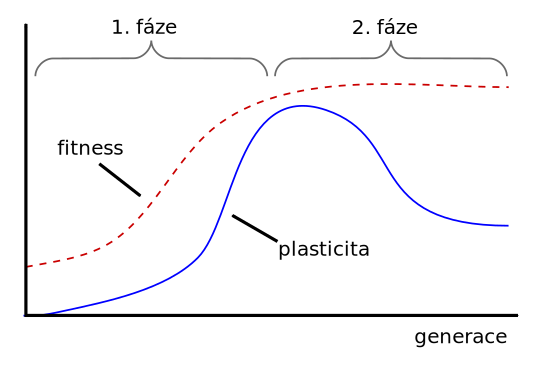
\includegraphics[width=0.5\textwidth]{fig/baldwinPlasticity.pdf}
    \caption{Baldwinův efekt -- nejprve jsou upřednostňování plastičtější jedinci, později převáží cena učení a plasticita klesá \cite{EllefsenBalancing}.}
    \label{obrBaldwin}
\end{figure}

\subsection{Baldwinův efekt v~evolučních algoritmech}

První výpočetní model Baldwinova efektu představili Geoffrey Hinton a Steven Nowlan \cite{HintonNowlan}. Pracovali s~populací jedinců o~20 genech, které mohly nabývat hodnoty \textbf{0}, \textbf{1} nebo \textbf{?}. Genotyp je interpretován jako nastavení 20 spínačů. Alely \textbf{1} a \textbf{0} znamenají, že je příslušný spínač zapnut nebo vypnut, pokud gen obsahuje hodnotu \textbf{?}, může jedinec se spínačem experimentovat. Cílem bylo sepnout všechny spínače. V~případě, že některý gen byl nastaven na \textbf{0}, měl jedinec minimální fitness ($f = 1$), pokud byly všechny geny nastaveny na \textbf{1}, získal jedinec maximální fitness ($f = 20$). Jedinci s~\uv{otazníkovými} alelami měli 1~000 pokusů na nalezení správného řešení a jejich fitness byla určena jako $f = 1 + 19 \frac{1000 - i}{1000}$, kde $i$ znamená počet využitých pokusů. Po 50 generacích se ukázalo, že jedinci mají v~průměru 11 genů nastavených na \textbf{1} a 9 genů mělo hondotu \textbf{?}. \uv{Nulové} geny byly poměrně rychle eliminovány s~průměrnou fitness $f = 11,6$. Bez užití učení (a \uv{otazníkových} alel) je očekávaná fitness $f = 1$, protože pravděpodobnost vzniku jedince se všemi geny nastavenými na \textbf{1} je velmi malá a fitness funkce nenabízí žádné vodítko, který jedinec je lepší a který horší (každý má buď maximální nebo minimální fitness), jak znázorňuje obrázek \ref{obrHintonNowlan}. Přidáním učení vznikne se fitness funkce \uv{vyhladí}.

\begin{figure}[htb]
    \centering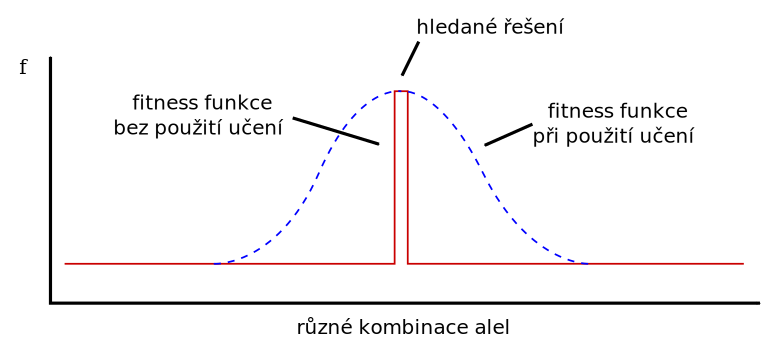
\includegraphics[width=0.7\textwidth]{fig/baldwin1.pdf}
    \caption{Fitness funkce z~experimentu Hintona a Nowlana \cite{HintonNowlan}.}
    \label{obrHintonNowlan}
\end{figure}

Byly představeny také modifikace kartézského genetického programování využívající plastických jedinců.
V~jedné z~nich chromozom obsahoval oproti standardnímu CGP jeden primární výstup navíc, který nebyl přímou součástí kandidátního řešení. U~nově vzniklých potomků je nejprve vytvořen fenotyp, který je posléze modifikován, dokud tento výstup není roven předem stanovené hodnotě. Fitness jedince je pak určena až pomocí modifikovaného fenotypu. V~experimentech na klasifikačních úlohách se ukázalo, že oproti standardnímu CGP lze dosáhnout menší chybovosti při klasifikaci testovací množiny dat \cite{UllahPlasticCGP}.

Jiným způsobem, jak spojit učení s~kartézským genetickým programováním, je odstranění genů kódujících  propojení primárních výstupů na funkční bloky z~chromozomu. Nově vzniklý jedinec pak experimentuje a hledá nejvhodnější funkční blok, jehož výstup bude sloužit jako některý z~primárních výstupů, tak aby dosáhl co nejvyšší fitness. Na úloze návrhu úplné sčítačky se ukázalo, že algoritmus končí úspěšně bez ohledu na velikost kartézské mřížky, zatímco u~standardního CGP úspěšnost s~větší mřížkou klesala. \cite{KhatirPlasticCGP}.

\subsection{Senzitivní období v~učení}

\blind
\blind

%\begin{itemize}
%    \item V případě, že je některý gen je nastaven na \textbf{0}

%V~situacích, kdy je prostředí relativně stabilní, lze očekávat, že chování původně získané učením se postupem času přenese do instinktů obsažených v~genotypu \cite{HowToShiftBias}.

%Na učení lze nahlížet jako na lokální prohledávání nad fitness funkcí v~okolí daného genotypu, fitness fenotypu je pak určena výsledkem tohoto prohledávání.

\chapter{Návrh obrazových filtrů pomocí souběžného učení}

Cílem této práce je navrhnout systém pro návrh obrazových filtrů založený na principech evolučních algoritmů, koevoluce a souběžného učení. Tento systém bude implementován a experimentálně vyhodnocen v~rámci diplomové práce.

Jedním z~nedostatků koevoluce s~prediktory fitness, popsané v~podkapitole \ref{secCoevIF}, je nutnost zvolit vhodnou velikost podmnožiny případů fitness, kterou vybírají prediktory. Tato velikost by měla být co nejmenší, aby byl počet nutných vyhodnocení co nejmenší, ale zároveň taková, aby odchylka mezi predikovanou a skutečnou fitness kandidátních řešení byla stále přijatelně nízká. Velikost vhodná pro jednu úlohu nemusí být vhodná pro jinou. Například v~případě symbolické regrese mohou u~jednoduchých rovnic stačit pouze jednotky trénovacích vektorů, u~obrazových filtrů to mohou být i tisíce. Někdy je pro stanovení optimální délky nutné provést velké množství experimentů s~různým nastavením; mohou to být i tisíce nezávislých běhů.

Další slabinou koevolučního návrhu je i problém škálovatelnosti -- u~složitějších úloh, jako je návrh obrazových filtrů, může prediktor čítat tisíce genů. Práce s~takto velkými genotypy je pak poměrně neefektivní.

Tyto nedostatky lze obejít použitím jiného kódování prediktorů, kdy nekóduje přímo ukazatele do množiny všech případů fitness, ale pouze návod, podle kterého se mají případy fitness vybírat. V~části \ref{secIndirectPredictors} je popsáno kódování prediktorů jako programy tvořené dle principů kartézského genetického programování, které generují posloupnost ukazatelů do množiny případů fitness, která může nabývat různé délky.

Tato práce se zabývá novým kódováním prediktorů, jehož cílem je tyto nedostatky zmírnit. Pokud umožníme tvorbu různě velkých prediktorů z~jednoho genotypu, mohou takto plastičtí jedinci reagovat jak na složitost právě řešené úlohy, tak na aktuální průběh evoluce.

Tato kapitola se nejprve v~části \ref{secDesignIF} zabývá evolucí obrazových filtrů, tvarem genotypu, způsobem tvorby nových jedinců a samotným průběhem evoluce. Kapitola \ref{secDesignPred} uvádí nový druh genotypu prediktorů fitness a způsob odvozování fenotypu jedince. Poslední část \ref{secDesignCoev} popisuje průběh koevoluce těchto prediktorů a obrazových filtrů.

\section{Evoluce obrazových filtrů}
\label{secDesignIF}

Obrazové filtry jsou vyvíjeny pomocí kartézského genetického programování, popsaného v~kapitole \ref{secCGP}. Chromozom tvoří vektor celých čísel kódující acyklický orientovaný graf. Jednotlivé funkční bloky jsou tvořeny trojicí genů -- první z~nich označuje prováděnou funkci, druhý a třetí gen pak určují, kam jsou připojeny jeho vstupy. Seznam funkcí, které mohou výpočetní uzly realizovat je v~tabulce \ref{tabCGPFunctions}. Programy mají devět primárních vstupů a jeden primární výstup. Na vstupy jsou přiváděny hodnoty pixelů z~9-okolí právě zpracovávaného pixelu, výstup udává novou hodnotu pixelu, tak jak je popsáno v~kapitole \ref{secIF}.

\begin{table}[htb]
    \begin{minipage}[t]{.5\textwidth}
        \centering\begin{tabular}{|c|l|l|}
            \hline
            \# & funkce & popis \\
            \hline
            0 & $255$ & konstanta \\
            1 & $i_1$ & identita \\
            2 & $255 - i_1$ & inverze \\
            3 & $i_1 \vee i_2$ & OR \\
            4 & $\neg i_1 \vee i_2$ & OR s~negovaným vstupem \\
            5 & $i_1 \wedge i_2$ & AND \\
            6 & $\neg (i_1 \wedge i_2)$ & NAND \\
            7 & $i_1 \oplus i_2$ & XOR \\
            \hline
        \end{tabular}

    \end{minipage}
    \begin{minipage}[t]{.5\textwidth}
        \centering\begin{tabular}{|c|l|l|}
            \hline
            \# & funkce & popis \\
            \hline
            8 & $i_1 \gg 1$ & posun vpravo o~1 bit \\
            9 & $i_1 \gg 2$ & posun vpravo o~2 bity \\
            10 & $\mathrm{swap}(i_1, i_2)$ & prohození 4 bitů \\
            11 & $i_1 + i_2$ & sčítání \\
            12 & $i_1 +^S i_2$ & saturované sčítání \\
            13 & $(i_1 + i_2) \gg 1$ & průměr \\
            14 & $\max(i_1, i_2)$ & maximum \\
            15 & $\min(i_1, i_2)$ & minimum \\
            \hline
        \end{tabular}

    \end{minipage}
    \caption{Seznam funkcí výpočetních uzlů. Převzato z~článku \cite{SikuPPSN}.}
    \label{tabCGPFunctions}
\end{table}

Vstupem algoritmu je zvolený obrázek poškozený šumem a tentýž obrázek v~původní podobě. Každé 9-okolí poškozeného pixelu a odpovídající nepoškozený pixel tvoří jeden případ fitness.

Na začátku je náhodně vytvořena počáteční populace a vypočtena fitness všech jedinců. Jedinec s~nejlepší fitness se stává rodičem následující generace. Ostatní jedinci jsou nahrazeni jeho kopiemi a několik jejich genů je pozměněno mutací. Mutace dodržuje pravidla zmíněná v~části \ref{secCGPEvo} s~tím rozdílem, že není povoleno na primární výstup připojit primární vstup. Takto vytvořená populace je opět ohodnocena fitness funkcí a algoritmus pokračuje výběrem rodiče a tvorbou další generace.

Fitness jedinců je vypočtena ve dvou krocích: nejprve jsou určeny aktivní bloky rekurzivním sestupem od výstupů programu, poté jsou vypočteny směrem od vstupů programu výstupy všech aktivních bloků a tím i celého programu.

\section{Prediktory fitness}
\label{secDesignPred}

Tato část se zabývá návrhem prediktorů s~plastickým fenotypem, u~kterých lze z~jednoho genotypu dle okolního prostředí odvodit různé fenotypy.

Chromozom je reprezentován jako vektor číselných ukazatelů do množiny případů fitness o~předem stanovené délce. Ačkoliv není žádoucí, aby prediktor obsahoval některé případy fitness vícekrát, jsou v~genotypu povoleny duplicitní hodnoty. Zamezit by jim šlo použitím například permutačního kódování, ale to je pro chromozomy o~tisících genech, jenž se dají u~návrhu obrazových filtrů očekávat, už poměrně neefektivní. Evoluce probíhá pomocí genetického algoritmu popsaného v~částí \ref{secGA} s~použitím jednobodového křížení a mutačního operátoru, který náhodně nahrazuje geny náhodně vygenerovanými hodnotami. Fitness prediktoru je dána následující funkcí:

\begin{equation}
    \label{eqDesignPredFitness}
    f \left( p \right) = \frac{1}{u} \sum\limits_{i=1}^{u} \left| f_{\mathit{exact}} \left( s \left( i \right) \right) - f_{\mathit{predicted}} \left( s \left( i \right) \right) \right|
\end{equation}

\noindent{}kde $f \left( p \right)$ je fitness prediktoru, $u$ počet filtrů použitích k~ohodnocení prediktoru, $f_{\mathit{exact}}$ označuje skutečnou fitness filtru $s_i$ a $f_{\mathit{predicted}}$ predikovanou fitness filtru $s_i$.

Plasticita je dosažena tím, že fenotyp netvoří všechny ukazatele přítomny v~genotypu, ale pouze jejich část. Fenotyp je z~genotypu tvořen postupným čtením genů od zvolené pozice (\emph{offsetu}). Pokud hodnota právě čteného genu není obsažena ve fenotypu, je do něj vložena, v~opačném případě se gen ignoruje. Poté je přečten další gen a proces se opakuje. Během tvorby fenotypu nejsou čteny úplně všechny geny -- jejich počet je určen hodnotou \emph{maxUsedGenes}, která je součástí prostředí. Pokud je při čtení dosaženo konce genotypu, ale nebyl ještě přečten potřebný počet genů, pokračuje se od jeho začátku. Příklad tvorby fenotypu za použití pěti genů z~deseti ukazuje obrázek \ref{obrFenotyp}.

\begin{figure}[htb]
    \centering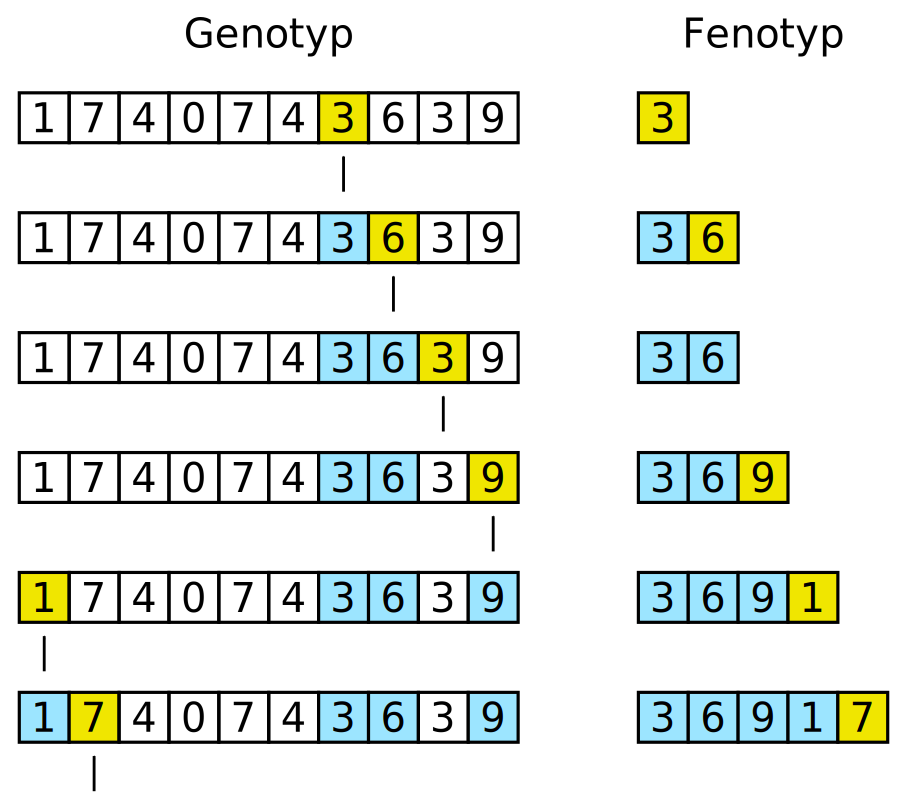
\includegraphics[width=0.45\textwidth]{fig/phenotype.pdf}
    \caption{Postup konstrukce fenotypu prediktoru. Šipka označuje právě přečtený gen.}
    \label{obrFenotyp}
\end{figure}

S~takto tvořenými jedinci lze experimentovat různými způsoby. Hlavním cílem práce je sledování průběhu evoluce a na základě posledních změn fitness nejlepšího filtru v~populaci upravovat hodnotu \emph{maxUsedGenes}. Předpoklady jsou následující:

\begin{itemize}
    \item Pokud fitness stoupá, je vhodné prodloužit prediktory a tím zpřesňovat predikci.
    \item Pokud se fitness nemění, evoluce pravděpodobně uvázla v~lokálním optimu a kratší prediktory mohou pomoci se z~tohoto optima posunout dále.
    \item Pokud fitness klesá, evoluce pravděpodobně opouští lokální optimum a mírné zkrácení prediktoru může pomoci postup urychlit.
\end{itemize}

Protože může délka prediktoru klesnout pod únosnou mez (v~extrémním případě to může být pouze jeden případ fitness), je součástí algoritmu také dolní mez nepřesnosti prediktoru, která je určena jako poměr mezi predikovanou a skutečnou fitness obrazového filtru. V~případě překročení této meze se délka prediktoru vždy zvýší bez ohledu na aktuální průběh evoluce.

S~plasticitou jedinců lze pracovat i dalšími způsoby. Například nově vytvořený prediktor může experimentovat s~offsetem a snažit se tak maximalizovat svou fitness -- tímto je simulováno jeho učení a přizpůsobování se prostředí. Další možností je v~situaci, kdy evoluce filtrů stagnuje, skokově změnit offset všech prediktorů v~populaci, což může pomoci v~posunu z~lokálního optima. Všechny zmíněné možnosti lze kombinovat.

\section{Koevoluce obrazových filtrů a prediktorů fitness}
\label{secDesignCoev}

Navrhovaný program pracuje na principech koevoluce popsané v~části \ref{secCoevIF}. Jeho součástí je populace obrazových filtrů, populace prediktorů fitness a archivy s~kandidátními filtry a prediktorem, který se používá k~ohodnocení filtrů. Navíc je zahrnut modul, který na základě průběhu evoluce rozhoduje o~změnách v~počtu genů, používaných pro tvorbu fenotypů prediktorů fitness (hodnota \emph{maxUsedGenes}).

\subsection{Fitness kandidátních filtrů}

U~populace obrazových filtrů jsou použity dvě různé fitness funkce. \emph{Skutečná fitness} je určena pomocí celé množiny případů fitness a slouží pro výpočet fitness prediktorů a také pro posuzování průběhu evoluce při modifikaci proměnné \emph{maxUsedGenes}. Oproti tomu \emph{predikovaná fitness} používá při výpočtu pouze případy fitness určené prediktorem. Používá se pro ohodnocení jak obrazových filtrů, tak prediktorů.

V~obou případech je fitness funkce obrazových filtrů špičková hodnota poměru signál/šum (Peak Signal to Noise Ration):

\begin{equation}
    \label{eqDesignPSNR}
    \mathit{PSNR} = 10 \log_{10} \frac{255^2}{\frac{1}{N} \sum\limits_i \left( v\left( i \right) - w\left( i \right)  \right)^2 }
\end{equation}

\noindent{}kde $N$ označuje počet použitých případů fitness, $v(i)$ a $w(i)$ pixel vyfiltrovaného (resp. původního) obrázku označený v~množině případů fitness indexem $i$.

\subsection{Archivy}

Obě populace se vyvíjejí souběžně v~oddělených vláknech a spolu interagují pouze prostřednictvím archivů. Archiv kandidátních filtrů je reprezentován kruhovým polem o~pevné délce. V~okamžiku, kdy je nalezen obrazový filtr s~lepší fitness, než měl jeho rodič, je umístěn do archivu. Také je uložena jeho skutečná fitness (určená pomocí všech případů fitness). Tyto filtry jsou poté použity pro výpočet fitness prediktorů dle rovnice \ref{eqDesignPredFitness}.

Archiv prediktorů je tvořen jedinou položkou -- nejlepším nalezeným prediktorem. Ten slouží k~výpočtu predikované fitness při evoluci obrazových filtrů.

\subsection{Sledování průběhu evoluce}

\chapter{Závěr}

\blind
\blind
 % viz. obsah.tex

  % Pouzita literatura
  % ----------------------------------------------

\ifczech
  %\bibliographystyle{czechiso}
\else
  \bibliographystyle{plain}
%  \bibliographystyle{alpha}
\fi
  \begin{flushleft}
  \printbibliography[title={Literatura}]
  %\inputencoding{latin2}
  %\bibliography{literatura-latin2} % viz. literatura.bib
  \end{flushleft}
  \appendix

  %\chapter{Obsah CD}
%\chapter{Manual}
%\chapter{Konfigrační soubor}
%\chapter{RelaxNG Schéma konfiguračního soboru}
%\chapter{Plakat}

\chapter{Uživatelská příručka}
\label{apxManual}

\chapter{Výsledky experimentů}
\label{apxResults}
 % viz. prilohy.tex
\end{document}
